\chapter{Locating API Misuse Examples in GitHub Data}
\label{cha:infoRetrieval}
This chapter provides an overview of the process used for extracting caveats from the Java 12 API documentation, extracting GitHub text and sample code data, and the use of NLP techniques (information retrieval systems) to perform sentence matching.  In particular, it was found that a significant lexical gap existed with API caveats and GitHub data, resulting in this approach to be unsuccessful. The purpose of this chapter is to, therefore, be a reference and act as a bridge for an alternative approach used in Chapter \ref{cha:codeAnalysis}. \bigbreak

\noindent
Section \ref{sec:info-intro} provides an overview of previously proposed methods for linking API caveats to code examples and how the same approach can be applied to GitHub. \bigbreak

\noindent
Section \ref{sec:info-design} describes TF-IDF, word2vec and BM25 as information retrieval systems alongside the architecture design of the approach for this chapter.\bigbreak

Section \ref{sec:info-implement} discuses the implementation process, which consists of the 
the extraction of GitHub data and API caveats from the Java 12 API documentation, and the process used for sentence matching via the creation of information retrieval systems. \bigbreak

\noindent
Section \ref{sec:info-results} discusses the findings of this chapter. \bigbreak

\section{Introduction}
\label{sec:info-intro}
One approach for linking API caveats to code examples is to utilise code examples provided by the programming community from Q\&A websites such as Stack Overflow. These websites allow users to post questions that contain some ``buggy'' code that requires fixing and have more experienced programmers provide suggestions or fixes. A core idea for linkage then involves locating questions that are related to API caveats and using their code examples as examples of API misuse. Note that conversely, the code examples from answer posts can be considered correct API usage samples. This can be achieved by measuring the lexical/semantic similarity between the natural language surrounding these code examples with the descriptions of API caveats. In particular, the method proposed by \cite{jiamou} and \cite{xiaoxue} uses sentence embedding to show that sentences in answer posts typically have high similarity to sentences of API caveats. Sentence embedding involves transforming sentences into some high dimensional vector space such that computers can ``understand'' them. For example, a sentence such as ``I like apples'' can be mapped to some sequence of numbers (a vector) that retains the original meaning of the sentence. The cosine similarity function can then be used to compute the cosine of the angle between two vectors. With sentence embeddings, the similarity function therefore outputs a score that represents the similarity of two sentences. This chapter aims to extend upon the previous approach by applying it to another domain: GitHub. \bigbreak

GitHub is a website that is abundant with community text and code examples, but its central focus is for providing an interface to a version control system (which is used to help developers maintain their projects over time). As a result, GitHub is commonly used for hosting free and open-source software and contains an abundance of code examples regarding many different APIs. According to GitHub's internal statistics\footnote{https://octoverse.github.com/}, the website includes over 31 million developers and 96 million project repositories in 2018. A key component of GitHub is its \textit{issues} features, which lets developers mainly report bugs for a repository (though it is also used to ask questions or make suggestions). Similar to a Q\&A website, these issues can contain multiple \textit{comments} from different users, that answers questions of the issue. Therefore, it can be seen that GitHub shares some similarities to Q\&A websites with the addition of a significantly larger collection of example code for analysis. The same approach from \cite{jiamou} and \cite{xiaoxue} can then be applied to GitHub to investigate if API caveat linkage to code examples can be improved with a different domain. \bigbreak

I extract 1,855,870 GitHub comments related to Java throughout 2018 via the GitHub Archive project. I then perform data cleaning and filtering to find comments associated with GitHub issues containing code examples, resulting in 629,933 comment sentences. Next, I data crawl the Java 12 API documentation to extract 73,831 API caveat sentences. I then perform similar text preprocessing and tokenisation to \cite{jiamou} to create 4 information retrieval systems consisting of TF-IDF, word2vec, BM25 and word2vec + BM25. This is used to match the API caveat sentences with GitHub comment sentences. I evaluate the information retrieval systems with a statistical random sampling method to compute the mean precision@3. However, all models performed considerably worse in comparison to the studies on Stack Overflow, with a mean precision@3 of 1\% or less. A significant lexical gap was identified as the cause of negative results. This was a consequence of the generic caveat sentences in the Java 12 documentation in combination with the fact that GitHub data relates to many different APIs, and fundamental differences in the community platforms.

\section{Design}
\label{sec:info-design}
Section \ref{subsec:info-tfidf} provides an overview of the TF-IDF statistic followed by a description of the word2vec model for sentence embedding (Section \ref{subsec:info-w2v}) and Okapi BM25 function (Section \ref{subsec:info-bm25}). Note that for these sections, \textit{documents} is used interchangeably with \textit{sentences} and \textit{terms} is used interchangeably with \textit{words}. An architecture design overview of this chapter is shown in Figure \ref{fig:github-architecture}. This resembles the architecture overview from \cite{jiamou}, with key differences in the \textit{Candidate Matching} step of the \textit{Matching Phase}. The differences include the use of several, different information retrieval systems in addition to an extension of the pure word2vec sentence embedding of the previous approach.

\begin{figure}
	\label{fig:github-architecture}
	\centering
	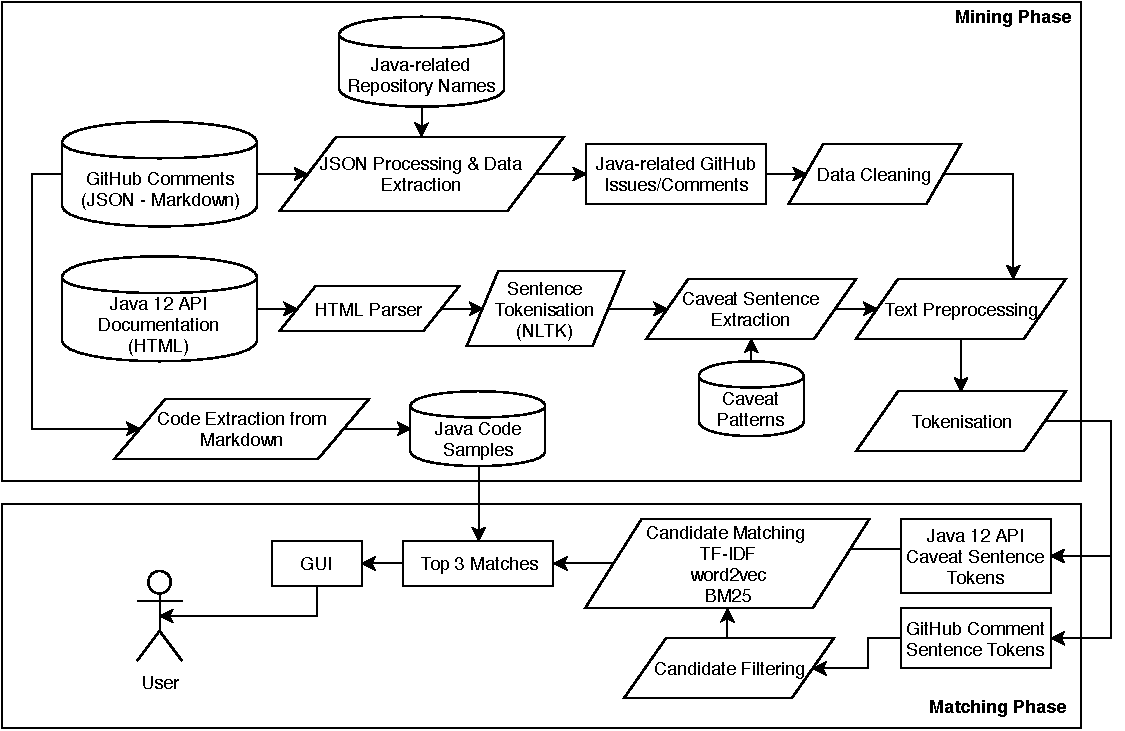
\includegraphics[width=0.8\textwidth]{figs/github-architecture.pdf}
	\caption{Architecture design of the work for this chapter.}
\end{figure}

\subsection{TF-IDF Sentence Matching}
\label{subsec:info-tfidf}
TF-IDF is short for \textit{term frequency-inverse document frequency}. TF is based on the frequency of a term within a document while IDF refers to the inverse of the number of documents that contain the given term \cite{robertson2004understanding}. TF-IDF is computed as $TF\cdot IDF$, which is the multiplication of two measures. The formal definition of IDF is shown in Equation \ref{idf}, where $t$ is a token and $D$ is the documents in the corpus (a collection of documents). The overall motivation for TF is based on the assumption that meaningful words tend to appear more often within a document. However, this assumption means common terms such as ``the'' and ``a'' would be incorrectly emphasised. The IDF is therefore used to minimise the weights of words that appear frequently across the entire corpus. \\
The TF-IDF heuristic is a widely used technique for information retrieval systems that have been successful in several cases \cite{tfidf-explain}. For sentences, TF-IDF typically follows a bag-of-words approach in which vectors have a length equal to the vocabulary size and each component of the vector corresponds to the TF-IDF score of a single term.

\begin{equation}
\label{idf}
idf( t, D ) = log \frac{ \text{| } D \text{ |} }{ 1 + \text{| } \{ d \in D : t \in d \} \text{ |} }
\end{equation}

\subsection{Word2Vec Embedding}
\label{subsec:info-w2v}
Word2vec involves a computationally efficient neural network that is trained to learn and produce word embeddings. The original motivation for this was to capture contextual information such that words could be predicted in a sequence of words \cite{mikolov2013efficient}. The two models that can be used with word2vec is Continuous Bag-of-Words (CBOW) and Skip-Gram, though only an overview of Skip-Gram will be provided as it is the model used for sentence embedding in this chapter. The Skip-Gram model effectively predicts surrounding words given the current word and has the property that ``simple vector addition can produce meaningful results'' \cite{mikolov2013distributed}. An example of this provided in \cite{mikolov2013distributed}. Suppose \textit{vec(x)} represents the vector form of word $x$, then vec(``Germany'') + vec(``capital'') would result in a vector close to vec(``Berlin''). A simple method for applying word embeddings to sentence embeddings is to use the sum of the word vectors of a sentence. This is the method used for sentence embeddings in \ref{subsec:info-candidate-match}.

\subsection{BM25 Ranking}
\label{subsec:info-bm25}
BM25 is a ranking function that outputs the relevance of documents in comparison to each other for a some query. It is computed from Equation \ref{eq:bm25}, where $f(q_i, D)$ is the term frequency of term $q_i$ (the $i^{th}$ term in document $D$), $|D|$ is the document length, $k_1$ and $b$ are tuning variables, and $IDF'$ is an alternative version of IDF that is defined by Equation \ref{eq:bm25-idf} \cite{Manning:2008:IIR:1394399}. In particular, $b=0.75$ and $k_1 \in [1.2,2]$ are reasonable values reported by \citeauthor{Manning:2008:IIR:1394399}. The values $b=0.75$ and $k_1$ were therefore used in \ref{subsec:info-candidate-match}. BM25 was considered a state-of-the-art model for information retrieval in previous years \cite{perez2009integrating}. It is noted that since the BM25 scores are only comparable for a specific query, they can be normalised to the range 0-1 with 0 representing the least amount of relevance and 1 representing the highest. This allows its ranking score to be used in conjuction with cosine similarity for sentence matching.

\begin{equation} \label{eq:bm25} 
\text{score}(D,Q) = \sum_{i=1}^{n} \text{IDF'}(q_i) \cdot \frac{f(q_i, D) \cdot (k_1 + 1)}{f(q_i, D) + k_1 \cdot (1 - b + b \cdot \frac{|D|}{\text{avgdl}})} 
\end{equation}

\begin{equation} \label{eq:bm25-idf} 
\text{IDF'}(q_i) = \log{\frac{N - n(q_i) + 0.5}{n(q_i) + 0.5}}
\end{equation}

\section{Implementation}
\label{sec:info-implement}
Implementation of the data retrieval and extraction of GitHub comments alongside Java 12 API caveats was completed in Python 3.6. In particular, the Gensim library was used to apply word2vec sentence embedding to GitHub comment sentences and Java API caveat sentences. The Sci-kit library was used to obtain sentence vectors from TF-IDF sentence embedding. Rankings for BM25 were computed manually using its associated function. Section \ref{subsec:info-github-extract} describes the collection of GitHub data and its extraction for sentence embedding and matching. Section \ref{subsec:info-caveat-extract} provides an overview of the Java 12 API documentation and extraction of its API caveat sentences. Section \ref{subsec:info-data-preprocess} explains the sentence preprocessing steps performed, followed by filtering steps to ease the scope of sentence matching required for the large sets of sentences (Section \ref{subsec:info-candidate-filtering}). Section \ref{subsec:info-sentence-embedding} illustrates the tools used for sentence embedding, and finally, Section \ref{subsec:info-candidate-match} describes how the Java 12 API caveat sentences were matched with sentences from GitHub comments.

\subsection{GitHub Data Extraction}
\label{subsec:info-github-extract}
There are three notable sources for GitHub data: (1) the GitHub Representational State Transfer (REST) API, (2) the GitHub Archive project, and (3) GitHub itself by cloning a repository. For this project, the GitHub REST API and GitHub Archive project was utilised due to the memory and processing requirements of cloning each repository of interest with option 3. However, the GitHub REST API contains several limitations that inhibit its usefulness for a large corpus of community text. This includes limitations on the request rate (30 requests per minute using the ``search'' API) and query options (e.g. it does not allow complex searches such as ``all GitHub issues associated with Java projects in January'', or more than 100 results per query). For option 2, GitHub Archive is a project that creates hourly archives of all GitHub data starting from 2/12/2011 as JSON objects. The archives include over 20 event types that are provided by GitHub such as the creation of an issue or comment. For issues and comments, the raw text of the posts is included in Markdown format, which represents the community text of interest.  However, these objects do not provide metadata for which programming languages or APIs are relevant. This makes it difficult to filter out irrelevant posts for information retrieval systems in later steps.
Thus, we combine the queries of the GitHub REST API to identify the repositories that are Java related, then link them with the community text captured by GitHub Archive.\bigbreak

In more detail, GitHub provides a REST API to allow developers to query for data on GitHub such as metadata about a particular repository or the number of repositories use some programming language. The REST API imposes a rate limit on user requests to prevent flooding of the GitHub servers. For this API, its  ``search'' functionality is the main solution for searching repositories or issues given specific conditions such as the time in which it was created. The API does not provide functionality to search for the contents of GitHub issues and comments across multiple repositories. Furthermore, the API is limited to a maximum of 100 results for a single query. The API is therefore only useful for finding which repositories contain Java code. The rate limit imposed is circumvented by performing numerous HTTP GET requests in sequence. This involves sending queries with a timer between each request and modified query parameters for (daily) creation times. A time window of 2009 to 2019 was chosen alongside a restriction of at least 2 ``stars'' to reduce the scope of projects collected to those that contained Java code and likely had more than 1 developer involved (as the number of stars a repository contains can be used to gauge its popularity). The PyGitHub Python library, in particular, is used to implement these queries to the GitHub REST API. Overall, collecting repository names of Java-related projects from 2009-2019 projects that contain at least 2 stars yields 291,152 results. \bigbreak

GitHub Archive captures an event known as ``IssueCommentEvent'', which contains various information about a comment for a particular issue. The archives are saved hourly. Therefore, a script is used to automate the process of downloading all archived data for 2018. Note that only data from 2018 is collected to reduce the amount of time required for querying the entire dataset and as an initial study. Multiprocessing is used in particular with a Python script to perform concurrent downloads and reduce the time required for data collection. After this, the extraction of relevant ``IssueCommentEvent'' objects is performed by checking whether the associated repository of a comment is Java related based on the list attained from the GitHub REST API. Notable information of these objects such as the text body of an issue comment and its title is extracted for natural language processing in later steps. Overall, this extraction process results in 627,450 GitHub issues and 1,855,870 issue comments to be collected.

\subsection{Java 12 Documentation Caveat Extraction}
\label{subsec:info-caveat-extract}
To begin extracting API caveats, the API documentation must first be collected. At the time of writing, the Java Standard Edition 12 API was chosen for analysis, which was the latest Java version and documentation available. This API was chosen as it comprises the standard library for Java and is, therefore, expected to be the most generalised API used by most Java projects. Its documentation consists of Hypertext Markdown Language (HTML) pages for each class of the Java Development Kit (JDK) 12. In particular, the API documentation contains a webpage in HTML that lists the complete class hierarchy tree of the Java standard library.\footnote{https://docs.oracle.com/en/java/javase/12/docs/api/overview-tree.html} This information allows us to data crawl the entire Java API documentation. First, the Uniform Resource Locator (URL) of all classes are mined from the class hierarchy page by collecting all hyperlink references on the page found within the appropriate HTML \lstinline{section} element. The Beautiful Soup/footnote{https://pypi.org/project/beautifulsoup4/} library is used to parse the HTML content. The relative URLs of each class are found by locating list item elements (\lstinline{li}) then anchor elements (\lstinline{a}) residing within. From this, absolute URLs are constructed for 4,865 classes. Next, the HTML pages for each class is downloaded by recursively sending HyperText Transfer Protocol (HTTP) GET requests for each of the URLs generated. A total of 4,712 classes are found. At this point, an important note to make for the Java SE 12 documentation is that it is automatically generated from comments in the source code implementation with the JavaDoc tool and is well-structured. For example, the parameters and possible exceptions for a method are consistently placed within certain HTML elements across all HTML pages. Hence, it is relatively simple to identify and extract sentences for each API element alongside additional information such as whether a method is deprecated from the existence of a \lstinline{div} element with the ``deprecationBlock'' Cascading Style Sheets (CSS) class for example.\bigbreak

The extraction of caveat sentences is performed by creating a set of regular expressions based on keywords and patterns identified in \cite{caveat-knowledge-graph}. These regular expressions allow us to check whether arbitrary strings contain some predefined patterns. API caveat sentences are then identified by checking if one of the regular expressions finds a match within a sentence from the API. This is executed recursively for all of the HTML pages, in which 115,243 caveat sentences are found. Of these sentences, 9,964 are regarded as \textit{class level sentences}, which are sentences that describe the overall class and are located in the class description section of API documents (typically at the top of each API document). A snippet of this is shown in Figure \ref{fig:class-sents}. The Java 12 API is also structured such that each method/field/constructor for a given class contains a self-contained section that describes details specific to that element. An example of this is shown in Figure \ref{fig:api-doc-eg}. We refer to the sentences that appear in the description of these sections as \text{element level sentences}. A total of 37,578 element level sentences are identified as caveat sentences. Other notable locations for sentences are sections that describe the parameters, exceptions or return value (if it is a method) of a particular API element. We refer to sentences found in those areas as \textit{parameter sentences}, \text{exception sentences} and \textit{return sentences} respectively. The total number of caveat sentences found at these levels is 67,701. Besides this, it is discovered that 1,522 API elements of the Java 12 API are deprecated. \\

\begin{figure}[h]
	\label{fig:class-sents}
	\centering
	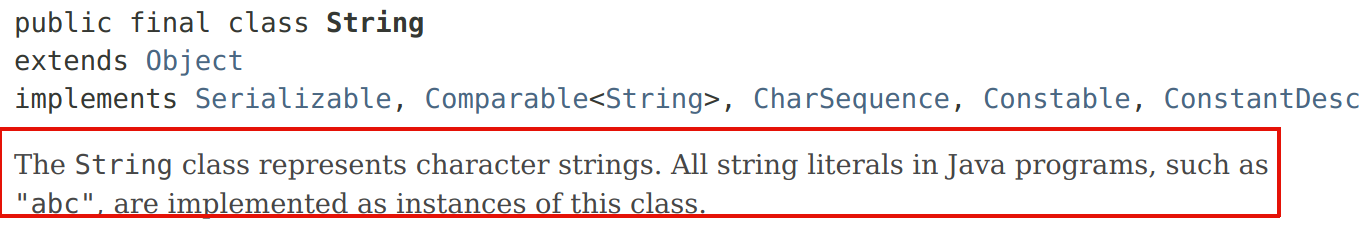
\includegraphics[width=\textwidth]{figs/class-sents-highlight.png}
	\caption{Example of the description section for the Java \lstinline{String} API documentation. Sentences located in this area (highlighted in red) are referred to as \textit{class level sentences}.}
\end{figure}

\begin{figure}[h]
	\label{fig:api-doc-eg}
	\centering
	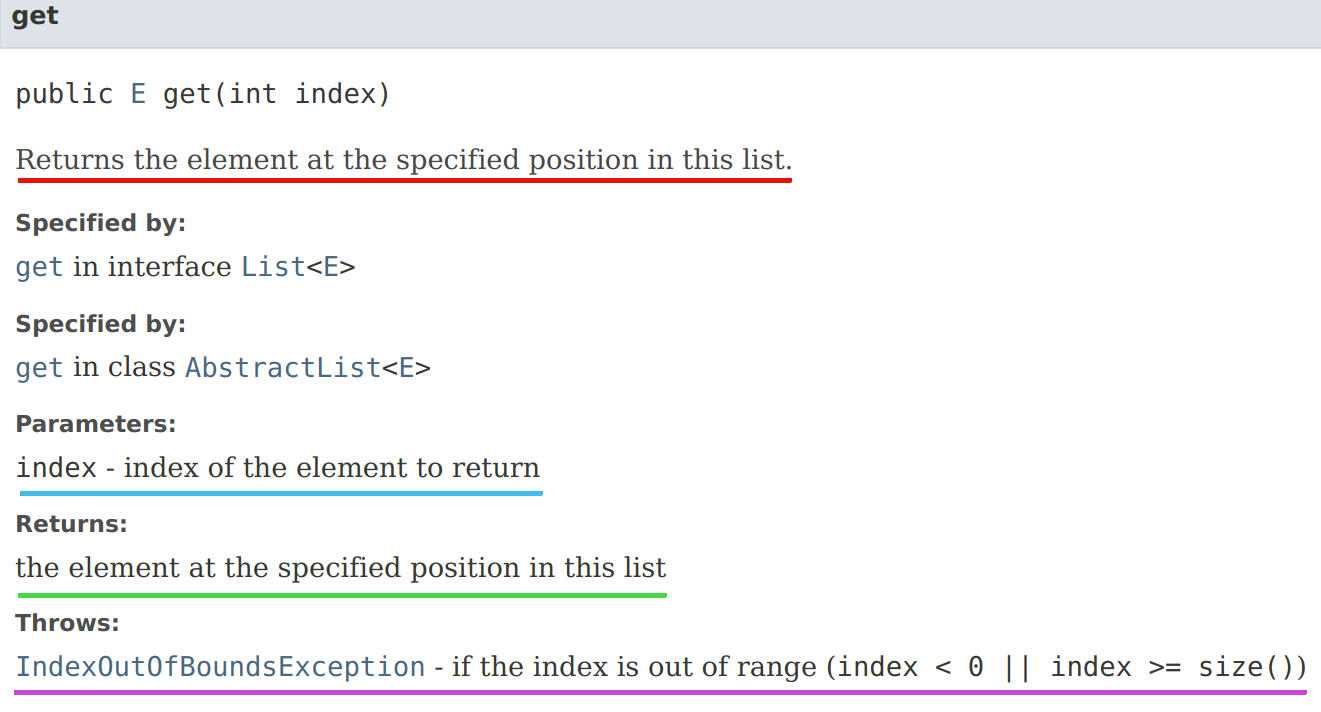
\includegraphics[width=\textwidth]{figs/api-doc-eg-highlight.png}
	\caption{Example of the API documentation for \lstinline{ArrayList.get(int index)}. Sentences located in the red underlined section, blue underlined section, green underlined section, and purple underlined section are referred to as \textit{element sentences}, \textit{parameter sentences}, \textit{return sentences} and \textit{exception sentences} respectively.}
\end{figure}

\begin{table}[]
	\centering
	\begin{tabular}{@{}lll@{}}
		\toprule
		\textbf{Category} & \textbf{Subcategory} & \textbf{Syntactic Pattern Examples} \\ \midrule
		\multirow{5}{*}{Explicit} & Error/Exception & \begin{tabular}[c]{@{}l@{}}``insecure'', ``susceptible'', ``error'',\\ ``null'', ``exception'', ``susceptible'',\\ ``unavailable'', ``not thread safe'',\\ ``illegal'', ``inappropriate'',\end{tabular} \\ \cmidrule(l){2-3} 
		& \multicolumn{1}{l}{Recommendation} & \multicolumn{1}{l}{\begin{tabular}[c]{@{}l@{}}``deprecate'', ``better/best to'',\\ ``recommended'', ``less desirable''\\ ``discourage''\end{tabular}} \\ \cmidrule(l){2-3} 
		& Alternative & ``instead of'',``rather than'',``otherwise'' \\\cmidrule(l){2-3} 
		& Imperative & ``do not'' \\\cmidrule(l){2-3} 
		& Note & ``note that'', ``notably'', ``caution'' \\\hline
		\multirow{2}{*}{Restricted} & Conditional & \begin{tabular}[c]{@{}l@{}}``under the condition'', ``whether ...'',\\ ``if ...'', ``when ...'', ``assume that ...''\end{tabular} \\\cmidrule(l){2-3}
		& Temporal & ``before'', ``after'' \\\hline
		\multirow{3}{*}{Generic} & Affirmative & \begin{tabular}[c]{@{}l@{}}``must'', ``should'', ``have to'',\\ ``need to''\end{tabular} \\
		& Negative & ``do/be not ...'', ``never'' \\
		& Emphasis & ``none'', ``only'', ``always'' \\ \hline 
	\end{tabular}
	\caption{API caveat categories and syntactic patterns from \cite{caveat-knowledge-graph}.}
	\label{tab:caveat-keywords}
\end{table}

\subsection{Data Preprocessing}
\label{subsec:info-data-preprocess}
Data cleaning and text preprocessing are required to allow NLP techniques/models to perform correctly. Numerous preprocessing steps are therefore applied to prepare the sentences for word and sentence embedding. In particular, the comments are in Markdown format, allowing simple removal of unwanted elements such as code blocks (which are wrapped between a pair of \lstinline{```}). Furthermore, all URLs, supplementary white space characters, apostrophes and punctuation (except for full stops appearing after a word) are removed. In particular, full stops are retained in consideration of inline code such as ``array.length''. The removed parts of the text are substituted with a white-space character so that individual components of references to API elements (e.g. ``array.length'') can be separated correctly during word tokenisation.  For sentence tokenisation, which separates a paragraph into its sentences, full stops that were followed by a space were used to identify the split points.  We note that a custom sentence tokeniser is required to prevent cases where full stops within inline code would result in a sentence split. Finally, word tokenisation is performed for each preprocessed sentence. This simply involves splitting the sentences based on white space characters such that each sentence is represented as a list of tokens. This representation is essential for further NLP tasks as it simplifies parsing/processing for computers. \bigbreak

Next is the removal of a customised set of English stop words provided by the NLTK library\footnote{https://www.nltk.org/index.html}. Stop words are common words that add little value/meaning for NLP such as ``a'' and ``is''. For the GitHub data, stop words that were of length 1 were retained such that single character variable names like ``i'' (commonly used by Java programmers in \lstinline{for} loops) are retained. Overall, preprocessing and tokenisation of all GitHub comments results in 1,855,870 tokenised sentences. It is noted here that in \cite{jiamou}, two additional steps are performed for the sentences: (1) coreference resolution, where pronouns such as ``it'' and ``this'' is substituted with the closest API names, and (2) lexicon construction in which an API lexicon (i.e. a vocabulary set of API element names) is constructed from the code of question and answer posts of Stack Overflow. Both of these steps are intended to reduce the complexity and noise of sentence embedding and matching. However, an initial search of the GitHub data via Google found that finding examples of API misuse from GitHub data is significantly more difficult than with Stack Overflow. For simplicity, step 1 is therefore ignored. Step 2 is reduced to keyword matching of both the API element name and its associated class name in Section \ref{subsec:info-candidate-filtering} when determining the relevant API elements of each GitHub comment, and hence, the list of potentially relevant API caveats for those comments.

\subsection{Candidate Filtering}
\label{subsec:info-candidate-filtering}
The caveat sentences that were associated with deprecated API elements or were not an element sentence, parameter sentence or exception sentence were filtered. In particular, the sentences for deprecated elements are ignored because those caveats are typically obvious to developers as Integrated Development Environments (IDEs), software that support programmers with development, highlight cases where an API element is deprecated. This is accomplished using the \lstinline{@Deprecated} annotation for Java that is tagged onto deprecated methods by API developers. I only focus on element, parameter and exception sentences to reduce the scope of sentences during sentence matching with GitHub comments and because these sentences were found to describe the most explicit caveats (such as  the ``index < 0 || index >= size()'' constraint in the exception sentence of Figure \ref{fig:api-doc-eg}). It is hypothesised that these explicit types of caveats are the most likely caveats to be matched to community sentences as they would require some form of paraphrasing to explain and would result in obvious errors and exceptions to be thrown.\bigbreak

For reference, it is observed that several caveat sentences extracted are invalid: they contain snippets of code or do not necessarily specify a constraint for users. Example of caveat sentences containing code snippets is shown in Listing \ref{invalid-caveat-1}, \ref{invalid-caveat-2} and \ref{invalid-caveat-3}. An example of an API caveat that does not specify a constraint is the class level sentence ``Java implementations must use all the algorithms shown here for the class Random, for the sake of absolute portability of Java code.'' from the \lstinline{Random} class/footnote{https://docs.oracle.com/en/java/javase/12/docs/api/java.base/java/util/Random.html}. To counteract sentences containing code snippets, those that exceeded an arbitrarily (generous) limit of 400 characters were excluded from further analysis and sentence matching. The other type of invalid caveat sentences were ignored as they appeared to represent a small portion of the extracted caveats.
In addition to this, it was noted that matching all of the GitHub issue comment sentences against every API caveat sentence would require significant processing time/power. The potentially relevant API caveats for each GitHub comment were therefore identified first to filter out non-relevant API caveats. This was achieved by concatenating the text of each comment and their associated GitHub issue, transforming the string to lowercase characters only, and performing a sub-string search for the (lowercase) class name and API element name of the API caveats. Caveats that were potentially relevant to more than 1000 GitHub comments were restricted to those 1000 GitHub comments to further reduce computation. This restriction involved 213 of the 21,932 API elements from the Java 12 documentation. We note that this limits the search area of sentence matching for those API caveats considerably, but is acceptable for an initial attempt of sentence matching. The total number of caveat sentences after preprocessing and all filtering  functions totalled 73,831.\bigbreak

For GitHub comments, those that were not attached to an issue containing a code block were filtered. This is because the overall purpose of sentence matching is to indirectly link API caveats to code examples. From the dataset, 85,318 issues contained a code block with  290,019 associated comments. Those comments contained 629,933 sentences in total. The next step for sentence matching was to perform sentence embedding.

\begin{lstlisting}[label=invalid-caveat-1,caption={An example of a caveat sentence extracted from the \lstinline{javax.swing.Spring} documentation containing some snippets of code or mathematical expressions},float,frame=tb,numbers=none,language=None,linebackgroundcolor={\lstcolorlines{4,5,6}}]
If we denote Springs as [a, b, c], where a <= b <= c, 
we can define the same arithmetic operators on Springs:

[a1, b1, c1] + [a2, b2, c2] = [a1 + a2, b1 + b2, c1 + c2]
-[a, b, c] = [-c, -b, -a]
max([a1, b1, c1], [a2, b2, c2]) = [max(a1, a2), max(b1, b2), max(c1, c2)]
\end{lstlisting}

\begin{lstlisting}[label=invalid-caveat-2,caption={An example of a caveat sentence extracted from the \lstinline{java.security.cert.X509CRL} documentation explaining the structure of a \lstinline{TBSCertList} object.},float,frame=tb,numbers=none,language=None,linebackgroundcolor={\lstcolorlines{3,4,5,6,7,8,9,10,11,12,13,14,15,16,17}}]
The ASN.1 definition of tbsCertList is:

TBSCertList  ::=  SEQUENCE  {
	version                 Version OPTIONAL,
	-- if present, must be v2
	signature               AlgorithmIdentifier,
	issuer                  Name,
	thisUpdate              ChoiceOfTime,
	nextUpdate              ChoiceOfTime OPTIONAL,
	revokedCertificates     SEQUENCE OF SEQUENCE  {
	userCertificate         CertificateSerialNumber,
	revocationDate          ChoiceOfTime,
	crlEntryExtensions      Extensions OPTIONAL
	-- if present, must be v2
	}  OPTIONAL,
	crlExtensions           [0]  EXPLICIT Extensions OPTIONAL
	-- if present, must be v2
}
\end{lstlisting}

\begin{lstlisting}[label=invalid-caveat-3,caption={An example of a caveat sentence extracted from the \lstinline{java.text.BreakIterator} documentation that contains some sample code.},float,frame=tb,numbers=none,language=None,linebackgroundcolor={\lstcolorlines{3,4,5,6,7,8,9,10,11,12,13,14,15,16,17}}]
Creating and using text boundaries:

public static void main(String args[]) {
	if (args.length == 1) {
		String stringToExamine = args[0];
		//print each word in order
		BreakIterator boundary = BreakIterator.getWordInstance();
		boundary.setText(stringToExamine);
		printEachForward(boundary, stringToExamine);
		//print each sentence in reverse order
		boundary = BreakIterator.getSentenceInstance(Locale.US);
		boundary.setText(stringToExamine);
		printEachBackward(boundary, stringToExamine);
		printFirst(boundary, stringToExamine);
		printLast(boundary, stringToExamine);
	}
}
\end{lstlisting}

\subsection{Sentence Embedding}
\label{subsec:info-sentence-embedding}
Sentence embedding provides a method of comparing the similarity of two sentences by representing them in vector space and computing the cosine similarity between the two vectors. Representing variable length sentences as fixed length vectors has been a major research topic related to deep learning approaches for NLP \ref{adi2016fine}.
For TF-IDF, the Scikit-learn library was used. This involved importing the class \lstinline{TfidfVectorizer} and calling its \lstinline{fit_transform} function to create vectors for all API caveat sentences. For word2vec sentence embedding, the \lstinline{word2vec} class from the \lstinline{gensim} library was imported and used. Note that the input for sentence embedding was the preprocessed, tokenised and filtered forms of caveat sentences from the previous sections. Overall, sentence vectors were generated via TF-IDF and word2vec functions/algorithms.

\subsection{Candidate Matching}
\label{subsec:info-candidate-match}
Sentence matching was accomplished using cosine similarity for the TF-IDF and word2vec sentence embedding vectors. For BM25, its function already output a ranking score and did not require further computation. To evaluate the cosine similarity of the vectors, each of the 73,831 caveat sentence vectors was compared to a subset of the 629,933 sentence vectors from GitHub comments corresponding to sentences deemed potentially relevant to the given caveat sentence in \ref{subsec:info-candidate-filtering}. The equation in \ref{cosine} was then used to compute the similarity scores. This score is then reversed such that 1 represents perfect similarity between two sentence vectors, while 0 represents complete dissimilarity between two sentence vectors. Given that BM25 ranks the sentence vectors relevant to each other, the scores were then normalised to the range 0 and 1, with 1 being representing highest similarity. Thus, scores were computed for each caveat sentence against their subset of potentially relevant GitHub comment sentences for TF-IDF, word2vec and BM25. A weighted combination of BM25 and word2vec was also considered (with equal weightings for both scores) since using both approaches could be expected to create a balance between their advantages and disadvantages. \\

\begin{equation}
\label{cosine}
\cos ({\bf A},{\bf B})= {{\bf A} {\bf B} \over \|{\bf A}\| \|{\bf B}\|} = \frac{ \sum_{i=1}^{n}{{\bf A}_i{\bf B}_i} }{ \sqrt{\sum_{i=1}^{n}{({\bf A}_i)^2}} \sqrt{\sum_{i=1}^{n}{({\bf B}_i)^2}} }
\end{equation}

To evaluate the performance of each of the approaches, a statistical sampling size was estimated via \ref{sample} using a 95\% confidence interval, 5\% error margin and a population size of 73,831 (i.e. the number of preprocessed and filtered caveat sentences). The estimated sampling size population was 383, though 384 was used for consistency with \cite{xiaoxue} in which notably more API caveat sentences from the Android documentation were analysed (160,112). The precision at K metric was chosen for a simplistic, initial evaluation of a query for the information retrieval systems, where K was set to 3 to reduce the amount of manual labelling required for all approaches (TF-IDF, word2vec, BM25 and word2vec combined with BM25). This would then be combined with the mean average precision (at k) to quantify overall performance of the systems across multiple queries. Therefore, a random sample of 384 caveat sentences was selected for each of the information retrieval systems and the top 3 results were returned for each query. Note that a random sample was computed for each system since we are mainly interested in relevant API caveat sentences are to GitHub data, and less on the performance of the systems. The different approaches are only used for a general idea of different approaches that can be compared to \cite{jiamou} where API caveat sentences from the Android documentation were linked to community answers on Stack Overflow. Considering cases in which the information retrieval systems can return less than 3 results, random sampling resulted in 959, 936, 1129 and 1051 results for the TF-IDF, word2vec, BM25 and word2vec + BM25 information retrieval systems for manual labelling.

\section{Results}
\label{sec:info-results}
Labelling for each of the information retrieval systems' results was conducted by manually checking if the given API caveat sentence query appeared to be relevant to the GitHub comment containing the matched sentence. The entire GitHub comment was used to include contextual information regarding the sentence, ensuring that the sentence was actually relevant to the API caveat. Thus, results were annotated with either \textit{relevant} or \textit{non-relevant} based on whether they referred to the API caveat query. It was found that a significantly small percentage of the results were relevant to their API caveat query, with only 9, 16, 5 and 11 results identified as relevant for the TF-IDF, word2vec, BM25 and word2vec + BM25 information retrieval systems. In other words, only about 1\% of the query results for the random samples were found to be relevant to their API caveats. The mean average precision at 3 for all of the information retrieval systems are therefore approximately 0. It was noted that using a similar version of the code on another (currently unpublished) work\footnote{\url{https://xin-xia.github.io/publication/ase192.pdf}} based on Stack Overflow and Android API caveats showed promising results. The results were therefore inspected to understand why the systems performed poorly for GitHub data.\\

\begin{lstlisting}[label=error-log,caption={Example of a GitHub comment containing an error log from \url{https://github.com/ChrisRM/material-theme-jetbrains/issues/863}},float,frame=tb,numbers=none,language=None]
similar problem just now, Linux (CentOS), upgrading from 2018.1 to 2018.2. 
(I use the Darcula theme, and this stack trace is suggestive...)\r\n\r\njava.lang.ClassCastException: java.lang.Boolean cannot be cast to com.intellij.openapi.actionSystem.ex.ComboBoxAction\r\n\tat com.intellij.ide.ui.laf.darcula.ui.DarculaButtonUI.
getComboAction(DarculaButtonUI.java:75)\r\n\tat com.intellij.ide.ui.laf.darcula.ui.DarculaButtonUI.
getDarculaButtonSize(DarculaButtonUI.java:236)\r\n\tat com.intellij.ide.ui.laf.darcula.ui.DarculaButtonUI.
...
\end{lstlisting}

From further analysis of the results, it was found that numerous GitHub comments contained code or error logs as text. In particular, error logs are common occurences as GitHub contains repositories for many different APIs and projects, though formatting of these are not regulated. An example of an error log for a GitHub comment in its raw text form is shown in \ref{error-log}. Note that the example has been truncated and long lines were split for better viewing. This would result in some of the code words to be processed as natural language words for the information retrievals and would also be difficult to clean. In addition, it was noted that GitHub contains a collection of text regarding many different APIs. In comparison to Stack Overflow, which allows users to tag their questions under a certain topic (such as Android), GitHub does not provide that functionality. This means it is much harder to differentiate the GitHub comments by API relevance. The consequence of this was seen from many cases where the correct API method name was identified, but because the name was quite generic (e.g. \lstinline{truncate}, \lstinline{compareTo}, \lstinline{getOffset}), the information retrieval systems would provide positive results for comments concerning caveats from other Java related APIs. It is noted that perhaps linking caveats for a more specific API (such as specific Java libraries like ReactiveX or OkHttp) would yield better results for GitHub since those projects have GitHub repositories that allow users to ask project/API related questions contained within their repositories. Furthermore, many of the caveat sentences from the Java API could be considered too generic. For example, the \lstinline{set} and \lstinline{get} methods of the \lstinline{java.util.ArrayList<E>} class both share the same sentence: ``IndexOutOfBoundsException - if the index is out of range (index < 0 || index >= size())''. An example where unrelated classes and methods of the Java API contain similar caveat sentences is from the constructor of \lstinline{java.util.HashMap<K,V>} that says ``NullPointerException - if the specified map is null'' and from the \lstinline{addAll} method of \lstinline{java.util.ArrayList<E>} that says ``NullPointerException - if the specified collection is null''. \\

Another possible reason that GitHub was considerably worse for linking API caveat sentences is because its community text serves a different purpose compared to Q\&A websites such as Stack Overflow. In particular, community text regarding API caveats would likely be in the format of a bug report, and answers to specific caveats can already be found on platforms catered to answering those caveats (i.e. Stack Overflow). Ultimately, it can be seen that due to the usage of same/similar sentences for different API elements, the inclusion of many different APIs on GitHub, and different purpose of GitHub results in a significant lexical gap for the Java 12 API caveat sentences and community text from GitHub. The poor results from this approach lead to the idea for a more direct approach of linking the API caveat sentences to source code described in Chapter \ref{cha:codeAnalysis}.

\section{Summary}
\label{sec:info-summary}
This chapter described the background work by \cite{jiamou} and \cite{xiaoxue} that is the approach used for linking API caveats to code examples. This chapter also focuses on extending the previous solutions to a different domain: GitHub. The data of GitHub is of interest for API caveat linkage because it is another community-centered website that contains an abundance of code. However, GitHub is inherently different from the focus of \cite{jiamou} and \cite{xiaoxue}, which was strictly Q\&A community websites. The Java 12 API documentation was used instead of the Android API documentation for API caveats as it could be generalised to more projects on GitHub. After extraction, 115,243 caveat sentences were found for the Java 12 API. For GitHub data, the GitHub Archive project was used to collect all GitHub events throughout 2018. The complete list of Java-related projects that had at least 2 stars was also collected using the GitHub REST API, finding 291,152 projects. A total of 1,855,870 GitHub comments related to Java in 2018 were then identified. The sentences underwent data preprocessing, filtering, and sentence embedding (TF-IDF and word2vec) to perform sentence similarity computations between the two datasets of GitHub comment sentences and Java 12 API caveat sentences. After filtering, this involved matching 73,831 caveat sentences with 629,933 sentences from GitHub comments.
Information retrieval systems were created based on TF-IDF, word2vec, BM25, and word2vec + BM25, with caveat sentences used as queries and query results being GitHub comment sentences, ranked according to their relevance. Manual labelling was performed to measure the performance of the information retrieval systems. A statistical random sampling method was used with a 95\% confidence interval and 5\% error margin. It was found that 1\% or less of the query results were found relevant for all of the information systems used. The cause of this was discussed and suspected as a result of the differences in GitHub as a community platform in comparison to Q\&A websites. GitHub data is also polluted with many different APIs that makes it harder to discern which API arbitrary text is associated to (if any).\\
In Chapter \ref{cha:codeAnalysis}, I take a more direct approach to linking API caveat sentences to code by transforming API caveat sentences into \textit{contracts} and conducting static code analysis.
